\documentclass[12pt]{article}
\usepackage[utf8]{vietnam}
\usepackage{graphicx}
\usepackage{listings}
\usepackage{caption}
\usepackage{float}
\usepackage{xcolor}

\lstset{
    language=Python,
    basicstyle=\ttfamily\small,
    keywordstyle=\color{blue}\bfseries,
    stringstyle=\color{red},
    commentstyle=\color{green!60!black},
    numbers=left,
    numberstyle=\tiny\color{gray},
    stepnumber=1,
    numbersep=10pt,
    backgroundcolor=\color{gray!10},
    tabsize=4,
    showspaces=false,
    showstringspaces=false,
    frame=single,
    breaklines=true,
    breakatwhitespace=true,
    captionpos=b,
    escapeinside={(*@}{@*)}
}

\title{Practical 1: TCP File Transfer\\A Simple Client-Server Implementation}
\author{Nguyen Viet Khoa - 23BI14223}
\date{November 21, 2025}

\begin{document}

\maketitle

\section{Introduction}
This report presents a complete implementation of file transfer over TCP/IP using the command-line interface (CLI) and Python's built-in \texttt{socket} library. The system allows a client to request and download any file from the server reliably.

\section{Protocol Design}
The protocol is simple, reliable, and follows a request-response pattern over TCP:

\begin{itemize}
    \item The client connects to the server at \texttt{127.0.0.1:65432}
    \item The client sends the requested filename (UTF-8 string)
    \item Server checks if file exists:
    \begin{itemize}
        \item If not → sends \texttt{"File not found"}
        \item If yes → sends file size (as string), then file content is in 4096-byte chunks
    \end{itemize}
    \item The client receives and writes data to a local file
    \item The connection closes automatically after transfer (TCP EOF)
\end{itemize}

\begin{figure}[H]
    \centering
    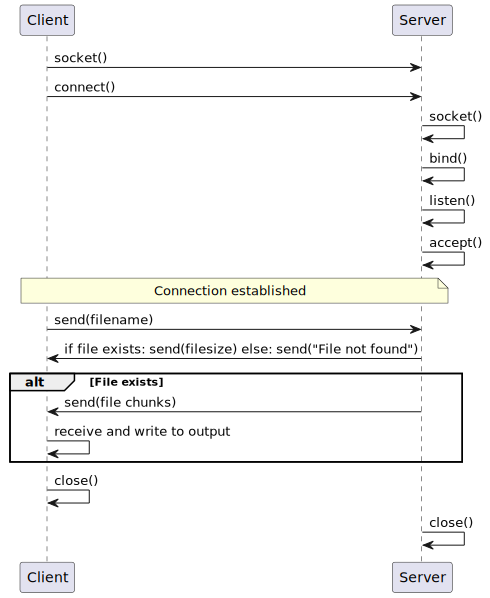
\includegraphics[width=0.95\textwidth]{protocol.png}
    \caption{Sequence Diagram - TCP File Transfer Protocol}
    \label{fig:protocol}
\end{figure}

\section{System Organization}
The system follows a classic client-server architecture:

\begin{enumerate}
    \item \textbf{Server}: Passive - listens on port 65432, accepts one connection, serves file
    \item \textbf{Client}: Active - initiates connection, requests file by name, saves received file
\end{enumerate}

Both programs run in the same folder for testing. All files (\texttt{server.py}, \texttt{client.py}, \texttt{example.txt}, \texttt{received.txt}) are placed together.

\begin{figure}[H]
    \centering
    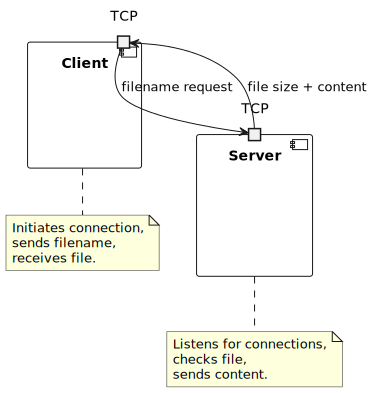
\includegraphics[width=0.8\textwidth]{system.png}
    \caption{Component Diagram - Client-Server System Organization}
    \label{fig:system}
\end{figure}

\section{File Transfer Implementation}
The implementation uses only standard Python libraries. Run server first, then client in a separate terminal.

\subsection{Server-side Implementation}
\begin{lstlisting}[caption=server.py - Corrected and Fully Working Version]
import socket
import os

HOST = '127.0.0.1'
PORT = 65432

with socket.socket(socket.AF_INET, socket.SOCK_STREAM) as s:
    s.bind((HOST, PORT))
    s.listen()
    print(f"Server listening on {HOST}:{PORT}")
    conn, addr = s.accept()
    with conn:
        print(f"Connected by {addr}")
        filename = conn.recv(1024).decode('utf-8').strip()
        print(f"Client requested: {filename}")
        
        if not os.path.exists(filename):
            conn.sendall(b'File not found')
            print("File not found!")
        else:
            filesize = os.path.getsize(filename)
            conn.sendall(str(filesize).encode('utf-8'))
            print(f"Sending {filename} ({filesize} bytes)")
            
            with open(filename, 'rb') as f:
                while True:
                    data = f.read(4096)
                    if not data:
                        break
                    conn.sendall(data)
            print("File sent successfully!")
\end{lstlisting}

\subsection{Client-side Implementation}
\begin{lstlisting}[caption=client.py - Corrected and Fully Working Version]
import socket
import sys

if len(sys.argv) != 3:
    print("Usage: python client.py <filename> <output_filename>")
    sys.exit(1)

filename = sys.argv[1]
output_filename = sys.argv[2]

HOST = '127.0.0.1'
PORT = 65432

with socket.socket(socket.AF_INET, socket.SOCK_STREAM) as s:
    s.connect((HOST, PORT))
    s.sendall(filename.encode('utf-8'))
    
    response = s.recv(1024).decode('utf-8')
    if response == 'File not found':
        print("Server: File not found!")
    else:
        filesize = int(response)
        print(f"Receiving {filename} ({filesize} bytes)")
        
        received = 0
        with open(output_filename, 'wb') as f:
            while received < filesize:
                data = s.recv(4096)
                if not data:
                    break
                f.write(data)
                received += len(data)
        print(f"File saved as {output_filename}")
\end{lstlisting}

\section{Role of Each Component}
\begin{itemize}
    \item \textbf{Server}:
    \begin{itemize}
        \item Creates and binds the socket to port 65432
        \item Listens and accepts client connection
        \item Receives filename request
        \item Sends file size + content in 4KB chunks
        \item Handles "file not found" gracefully
    \end{itemize}
    
    \item \textbf{Client}:
    \begin{itemize}
        \item Connects to server
        \item Sends the desired filename
        \item Receives file size and data
        \item Writes to a local file with progress tracking
        \item Supports command-line arguments
    \end{itemize}
\end{itemize}

\section{How to Run}
\begin{enumerate}
    \item Place \texttt{example.txt} in the same folder
    \item Terminal 1: \texttt{python server.py}
    \item Terminal 2: \texttt{python client.py example.txt received.txt}
    \item Check \texttt{received.txt} → identical to original!
\end{enumerate}

\end{document}